\chapter{The Standard Model and the charm-Yukawa coupling}
\label{chap:Theory}
In this chapter, the theoretical underpinnings of the analysis presented in this work are discussed. This includes a brief discussion of the SM in \autoref{sec:TheSM}, after which the charm-Yukawa coupling is introduced in \autoref{sec:CharmYukawa}. Following this, the cH process is discussed along with how it may be targeted by experiments such as the CMS detector \autoref{sec:measuringYc}. Finally, an effective field theory (EFT) interpretation of the cH process is discussed in \autoref{sec:cHEFT}.


\section{The Standard Model of particle physics}
\label{sec:TheSM}
The SM is formulated through the formalism of Quantum Field Theory (QFT). This is a formalism that combines concepts of classical field theory, quantum mechanics as well as special relativity into a single, coherent description of fundamental particles as excitations of underlying fields that pervade space-time. In this description, SM particles fall into two categories: fermions and bosons. The former are the massive particles which make up the matter of the universe while the latter are the force-carrying particles of the strong and electroweak forces. The distinction between these categories is made based on the spin of the particle, which may be of either half-integer or integer, respectively. \\
\\
The fermion content of the SM consists of 12 unique particles. These include six leptons, namely the electron, muon and tau as well as their respective neutrinos alongside six different quarks that are distinguished by their so-called \textit{flavour}. The different quark flavours include up, down, charm, strange, bottom and top, which specify a quark's mass eigenstate as well as electric charge. These fermions are typically arranged into three generations depicted as

\begin{align}
        \begin{pmatrix}
            e \\
            \nu_{e}
        \end{pmatrix}
        \begin{pmatrix}
            \mu \\
            \nu_{\mu}
        \end{pmatrix}
        \begin{pmatrix}
            \tau \\
            \nu_{\tau}
        \end{pmatrix}
        \, , \,
        \begin{pmatrix}
            \, u \, \\
            \, d \,
        \end{pmatrix}
        \begin{pmatrix}
            \, c \, \\
            \, s \, 
        \end{pmatrix}
        \begin{pmatrix}
            \, t \, \\
            \, b \,
        \end{pmatrix}.
\end{align}
\\
There are distinct differences between the leptons and quarks. Leptons carry integer (or no) electrical charge while quarks carry fractional electrical charges. More importantly, while both quarks and leptons may interact via the electroweak force, only the quarks interact via the strong force. A special feature of the strong force is that the potential energy associated with it grows as the distance between strongly interacting particles increases. This leads to a phenomenon referred to as \textit{confinement}, where quarks almost exclusively form compositive states called \textit{hadrons}. As a result, the emission of individual quarks or \textit{gluons} (the force carrying particles of the strong force) in scattering processes typically produce complex cascades of particles referred to as \textit{jets}, where the individual particles will ultimately form a variety of hadrons in a process referred to as \textit{hadronisation}. This gives rise to a very complex phenomenology of proton-proton (pp) collisions such as those at the LHC. At very high energies, the processes that involve the strong force, typically referred to as quantum chromodynamics (QCD) processes, can be understood through perturbative descriptions. This refers to an expansion of the expressions that describe QCD processes in the strong coupling constant $\alpha_{\mathrm{s}}(Q^2)$, which has an inverse scaling relationship with the momentum transfer of a process $Q$. As a result, $\alpha_{\mathrm{s}}(Q^2)$ becomes larger at lower energies and phenomenological descriptions are relied on in this regime instead. \\
\\
Lastly, the existence of anti-fermions must be mentioned. These carry the exact opposite quantum numbers (e.g. charge) as their fermion counterparts, though otherwise behave similarly (take the electron and positron for instance). For simplicity, references to a fermion in this work may be understood as referencing both the fermion and anti-fermion counterpart, unless otherwise indicated explicitly. Examples of the latter are e.g. referring explicitly to electrons e$^{-}$ and positrons e$^{+}$ or charm quark c and anti-charm quark $\bar{\mathrm{c}}$ pairs. \\
\\
There exist 13 unique bosons in the SM. These include the photon $\gamma$, W$^{\pm}$ and Z which mediate the electroweak force as well as 8 gluons $g$ that mediate the strong force. The final piece is the Higgs boson. Contrary to the force carriers, which all are spin 1, the Higgs boson is spin 0. The massive particles of the SM acquire their mass by interacting with the BEH field, excitations of which are identified as the Higgs boson particle, and is therefore a central element of the SM. \\
\\
Considering the introduced particles and forces, the SM has a rich and detailed phenomenology. A great example of a mathematically rigorous delineation of this can be found for example in \cite{PeskinSchroeder}. Given the focus of this work on the Yukawa coupling between the Higgs boson and charm quark, only this aspect of the SM is discussed in further detail.

\section{The charm-Yukawa coupling}
\label{sec:CharmYukawa}
The quantity that defines the strength of the interaction between massive fermions and the Higgs boson is the so-called Yukawa coupling. To better understand this and associated concepts, some knowledge of the electroweak sector of the SM is required. These are discussed in this section while a comprehensive overview may be found in \cite{WolfHiggs}. \\
\\
To understand the origin of the Yukawa couplings, a brief discussion of Lagrangian densities, gauge transformations and the role of symmetries in the SM is useful. The Lagrangian density \Lagr($\phi_i$; $a_i$) is a quantity dependent on a set of fields $\phi_i$ and constants $a_i$ from which the equations of motions for the particles associated with these fields may be derived. Commonly, theories of particles and their behaviour in a QFT are therefore defined through the formulation of a Lagrangian density. The form of this expression determines the nature of the particles that are included as well as their interactions. \\
\\
The concept of gauge symmetries is a central component to the way in which particle interactions are introduced in the Lagrangian formulation of the SM. These originate from the fact that the quantum fields in a QFT carry phase information, which may depend on the space-time coordinate of the field. This phase information describes (local) degrees of freedom of the field and should have no effect on the physical observables of the system. Accordingly, the Lagrangian \Lagr \, that describes the system, should remain invariant under arbitrary phase transformations. These transformations are typically referred to as a choice of gauge and the corresponding invariance is accordingly referred to as a \textit{local gauge symmetry}. \\
\\
In the Lagrangian of the SM, invariance in the presence of local gauge symmetries is ensured through the addition of gauge fields. These gauge fields couple to the previously existing fields and effectively serve as mediators of phase information between space-time points of the original fields. It is exactly these gauge fields that we identify as the fields describing the previously introduced force-mediating bosons, and which are required to maintain local gauge symmetry. A very interesting conclusion from this is that the dynamics of the bosons and the corresponding force are determined entirely by the structure of the local gauge symmetry that must be preserved. For the electroweak force, the corresponding symmetry is referred to as $SU(2)_{L} \, \mathrm{x} \, U(1)_{\mathit{Y}}$.  Here, the $L$ refers to the fact the weak force, described by the $SU(2)_{L}$ symmetry, only acts on left-handed particles. The handedness of particles, also referred to as the \textit{chirality}, originates from the relativistic description of particles in space-time using the Poincar\'{e} symmetry group. Specifically, this group is used to describe the underlying symmetries of special relativity, namely the symmetries associated with translations, rotations and boosts. A physical interpretation of chirality  can be gained by considering a massless particle's \textit{helicity}, which is the projection of the particle's spin onto its momentum vector. When the direction of the particle's spin coincides with the particle's momentum, it is considered to be right-handed. Accordingly, when the direction of the particle's spin is in the opposite direction of the momentum, it is considered to be left-handed. This, however, only holds true for massless particles, since for massive particles the helicity can change depending on an observer's frame of reference. Since the weak force makes a distinction based upon a particle's chirality, left and right-handed particles are represented in different ways in its formulation. These representations are referred to as doublets and singlets, respectively. In total, there are four bosons associated with the electroweak force. These are the photon $\gamma$, which mediates the electromagnetic force, as well as the electromagnetically charged W$^{\pm}$ and electromagnetically neutral Z boson that mediate the weak force. \\
\\
With these concepts in mind, the nature of the electroweak sector's Lagrangian in the SM may be discussed. Naively, the form of this would be given by

\begin{align}
    \label{LEWK} 
    \mathcal{L}_{\mathrm{EW}}= &i \overline{\psi}_L \gamma^{\mu} D_{\mu}^L \psi_L + i \overline{\psi}_R \gamma^{\mu} D_{\mu}^R \psi_R
    - \frac{1}{2} \mathrm{Tr} \left(W_{\mu\nu}^{a}W^{a\mu\nu} \right) 
     - \frac{1}{4} B_{\mu\nu}B^{\mu\nu} \, ,
\end{align}
\\
for a generic combination of a left-handed doublet $\psi_L$ and right-handed singlet $\psi_R$. The individual elements of $\mathcal{L}_{\mathrm{EW}}$ are briefly summarised below:
\\
\begin{align*}
    &g^{\prime}: &\mathrm{coupling}\, \mathrm{constant} \, \mathrm{of} \, \mathrm{U(1)}_Y \\
    &g: &\mathrm{coupling}\, \mathrm{constant} \, \mathrm{of} \, \mathrm{SU(2)}_L \\
    &\psi_L, & \textrm{left-handed} \, \mathrm{doublet}\\
    &\psi_R,  &\textrm{right-handed} \, \mathrm{singlet} \\
    &B_{\mu}: &\mathrm{gauge} \, \mathrm{field}\, \mathrm{of} \, \mathrm{U(1)}_Y\\
    &W_{\mu}^a : &\mathrm{gauge} \, \mathrm{fields} \, \mathrm{of} \, \mathrm{SU(2)}_L, \, a = 1,2,3 \\
    &W_{\mu\nu}: &\mathrm{field}\, \mathrm{strength}\,  \mathrm{tensor} \\
    &B_{\mu\nu}: &\mathrm{field}\, \mathrm{strength}\,  \mathrm{tensor} \\
    &t^{a} = \frac{\sigma^{a}}{2}, &\mathrm{SU(2)}\, \mathrm{generators} \\
    &Y_L = -1, &\mathrm{left} \, \mathrm{chiral} \, \mathrm{hypercharge}\\
    &Y_R = -2, &\mathrm{right} \, \mathrm{chiral} \, \mathrm{hypercharge}\\
    &D_{\mu}^L = \partial_{\mu}+ig^{\prime} \frac{Y_L}{2}B_{\mu}+igt^{a}W^{a}_{\mu}\\
    &D_{\mu}^R = \partial_{\mu}+ig^{\prime} \frac{Y_R}{2}B_{\mu}\\
\end{align*}
\\
The terms $D_{\mu}^{L/R}$ are so-called covariant derivates that ensure the local $\mathrm{SU}(2)_L \, \mathrm{x} \, \mathrm{U}(1)_{Y}$ gauge symmetry is upheld for $\mathcal{L}_{EW}$. These contain the coupling constants $g^{\prime}$ and $g$, which determine the coupling strength of fermions to the $B_{\mu}$ and $W^{a}_{\mu}$ gauge fields, respectively. The generators of the SU(2)$_{L}$ group are the Pauli matrices, with which arbitrary SU(2)$_{L}$ gauge transformations may be described. Finally, the left and right chiral hypercharges are the charges associated with the $U(1)_{\mathit{Y}}$ symmetry of the electroweak force. Further details can be found in \cite{WolfHiggs}. \\
\\
In this formulation, the observed charged gauge bosons W$^{\pm}$ arise from linear combinations of the $W_1$ and $W_2$ gauge fields
\begin{align}
    W^{\pm} = \frac{1}{\sqrt{2}}(W_1 \mp iW_2) , 
\end{align}
while the Z boson and photon $\gamma$ arise from linear combinations of the $W_3$ and $B$ gauge fields achieved via a rotation
\begin{equation}
    \begin{pmatrix}
    \gamma \\
    Z
    \end{pmatrix} = 
    \begin{pmatrix}
    \mathrm{cos}\theta_{\mathrm{W}} & \mathrm{sin}\theta_{\mathrm{W}} \\
    \mathrm{-sin}\theta_{\mathrm{W}} & \mathrm{cos}\theta_{\mathrm{W}}
    \end{pmatrix}
    \begin{pmatrix}
    B \\
    W_3
    \end{pmatrix} \,
\end{equation}
with the weak mixing angle $\theta_{\mathrm{W}}$. \\
\\
The massive natures of the W$^{\pm}$ and Z bosons, first reported in \cite{WZMass}, are however incompatible with such a formulation. The reason is that naive mass term such as 
\begin{align}
    m_W^{2}W_{\mu}^{+}W^{-, \mu}+\frac{1}{2}m_Z^{2}Z_{\mu}Z^{\mu}. \label{NaiveWZMass}
\end{align}
\\
do not remain invariant under arbitrary $\mathrm{SU(2)_L}$ gauge transformations. This is as gauge fields $A_{\mu}$ generically transform as 

\begin{align}
    A_{\mu} \rightarrow A_{\mu}^{'} =  A_{\mu} - \frac{1}{g} \partial_{\mu} \mathcal{V}(x), \label{FieldTransform}
\end{align}
\\
where $\mathcal{V}(x)$ is some arbitrary phase depending on the spacetime coordinate $x$. Substituting \autoref{FieldTransform} into \autoref{NaiveWZMass} thus introduces additional terms that do not cancel. The same is true for fermion mass terms in the form of
\begin{align}
    m_{f}\overline{\psi}\psi. \label{NaiveFermionMass}
\end{align} 
\\
Here, the invariance breaking terms arise from different transformation behaviours of $\psi_{L}$ and $\psi_{R}$ under $\mathrm{SU}(2)_L \, \mathrm{x} \, \mathrm{U}(1)_{Y}$ gauge transformations, since the $\psi_{L}$ component participates in the weak force while $\psi_{R}$ does not. 
\subsection{The Brout-Englert-Higgs mechanism}
The BEH mechanism provides a way to circumvent the gauge symmetry breaking nature of the aforementioned mass terms. This is achieved through a process referred to as \textit{spontaneous symmetry breaking}. A spontaneously broken symmetry refers to a symmetry that is upheld in a global view of the system (i.e. the overall Lagrangian density $\mathcal{L}_{\mathrm{EW}}$ remains invariant under a relevant gauge transformation) while the energetic ground state of the system explicitly breaks this symmetry. This is a process formally described by the Goldstone theorem \cite{Goldstone}, which states that each broken symmetry in a relativistic QFT generates an additional massless boson. These introduce additional degrees of freedom into the theory and are coined Goldstone bosons. The BEH mechanism exploits this by adding the term
\begin{align}
        \mathcal{L}_{\mathrm{Higgs}} &= D_{\mu} \phi^{\dagger} D^{\mu} \phi - V(\phi) \label{HiggsTerm} \\
        V(\phi) &= - \mu^{2}\phi^{\dagger} \phi + \lambda(\phi^{\dagger}\phi)^2 \label{HiggsPotential} 
\end{align}
to $\mathcal{L}_{\mathrm{EW}}$, that describes an additional complex field $\phi$. This is a SU(2)$_{L}$ doublet 
\begin{align}
    \phi= \begin{pmatrix}
        \phi^{+} \\
        \phi^{0}
        \end{pmatrix} 
\end{align}
with the scalar components $\phi^{+}$ and  $\phi^{0}$. Here, $V(\phi)$ corresponds to the potential energy term of the field. Again, the covariant derivative 
\begin{align}
    D_{\mu} = \partial_{\mu}+ig^{\prime}\frac{Y_{\phi}}{2}B_{\mu}+igt^{a}W_{\mu}^{a}
\end{align}
ensures $\mathcal{L}_{\mathrm{Higgs}}$ remains locally gauge invariant under $\mathrm{SU}(2)_L \, \mathrm{x} \, \mathrm{U}(1)_{Y}$ transformations and therefore introduces couplings between the $\phi$ field and the $B_{\mu}$ and $W_{\mu}$ fields. The constants of the potential term \autoref{HiggsPotential} are chosen in such a way that the ground state of $V(\phi)$ is non-zero. This can be achieved by choosing them such that $\lambda >$ 0 and $\mu^{2} >$ 0. The result is a ground state of $V$ that is identified as the vacuum expectation value 
\begin{align}
    v=\sqrt{\frac{\mu^{2}}{2\lambda}} \, .
\end{align}
The center of the potential is now an unstable local maximum and the only stable configuration can be found in the non-zero ground state. This is demonstrated visually in \autoref{fig:HiggsPotential}. Through this, the symmetry of the potential is effectively broken. A popular choice of gauge for $\phi$ is 

\begin{align}
    \phi= \begin{pmatrix}
        0\\
        v + \frac{h}{\sqrt{2}}
        \end{pmatrix},
\end{align}
\\
where $h$ is a new scalar field that is used to parametrise radial perturbations of the potential's ground state. This choice is referred to as the unitary gauge and $h$ is identified as the field corresponding to the physical Higgs boson. By expanding \autoref{HiggsTerm} with this choice of $\phi$, a range of terms are introduced to $\mathcal{L}_{\mathrm{EW}}$. These contain a variety of interaction terms between the gauge fields and the Higgs field, as well as newly generated mass terms for the Z and W bosons

\begin{align}
    \left(\frac{g}{2}\right)^{2}v^{2}W_{\mu}^{+}W^{\mu-} &=m_{\mathrm{W}}^{2}W_{\mu}^{+}W^{\mu-} \\
    \left(\frac{\sqrt{g^{2}+g^{\prime}}}{2}\right)^{2}v^{2}Z_{\mu}Z^{\mu} &= m_{\mathrm{Z}}^{2}Z_{\mu}Z^{\mu} \, .
\end{align}
\\
This can be understood to mean that the electroweak coupling constants $g$ and $g'$ along with $v$ effectively determine the mass of the Z and W$^{\pm}$ bosons. A full description and compilation of all the terms of the electroweak Lagrangian density of the SM can be found in \cite{WolfHiggs}.

\begin{figure}
    \centering
    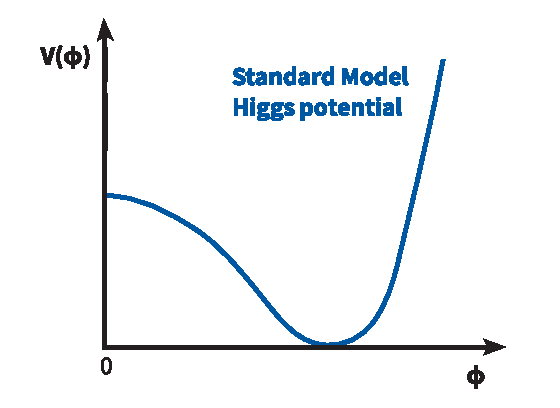
\includegraphics[width=0.6\textwidth]{figures/Higgs_potential.pdf}
    \caption{A sketch of the shape of the Higgs potential in the Standard Model, which is simplified by showing a cross section of the two-dimensional potential. A non-stable maximum at the center of a potential can be seen alongside a stable configuration in a non-zero ground state.}
    \label{fig:HiggsPotential}
\end{figure}

\subsection{The Yukawa couplings}
By including this additional contribution in our theory, mass terms for fermions may now be generated by including a term of the form
\begin{align}
    \mathcal{L}_{\mathrm{Yukawa}} &= -y_{f}\overline{\psi}\phi\psi \\
    &= -y_{f}v\overline{\psi}\psi(1 + \frac{1}{v}\frac{h}{\sqrt{2}}). \label{YukawaLagrangian}
\end{align}
This expression remains invariant under $\mathrm{SU}(2)_L \, \mathrm{x} \, \mathrm{U}(1)_{Y}$ gauge transformations due to the presence of $\phi$. Similarly to the W and Z mass terms, the relation
\begin{align}
    m_{f} = y_{f} v
\end{align} 
is obtained. A curious feature of the SM is that the Yukawa couplings $y_{f}$ are free parameters of the theory. As a result these must be measured experimentally, with the measurement of the charm-Yukawa coupling $y_{\mathrm{c}}$ being the goal of this work. Since the charm quark mass has previously been determined from experiment to be $m_{\mathrm{c}} = 1.27$ GeV \cite{PhysRevD.110.030001}, a measurement of $y_{\mathrm{c}}$ thus represents an important consistency test of the SM. To this end, one can exploit that an interaction between fermions and the Higgs field is introduced, as is evident from \autoref{YukawaLagrangian}, with an interaction strength proportional to $y_{\mathrm{c}}$. It is this feature that may be utilised by experiments at the LHC to measure $y_{\mathrm{c}}$. The presence of such interactions is also how other Yukawa couplings, such as of the bottom and top quarks, are determined experimentally and have been found to be consistent with the SM expectation \cite{bottomYukawa}\cite{topYukawa}. 
\section{Measuring the charm-Yukawa coupling}
\label{sec:measuringYc}
By measuring the frequency of occurrence of physics processes in which the coupling between the Higgs boson and charm quark appears, $y_{\mathrm{c}}$ may be determined. As such, a suitable process must be found that can be detected by an experiment such as the CMS experiment, which records pp collisions at the LHC. As previously introduced, these fall into three general categories. The first consists of the inclusive Higgs boson production process. This encompasses a range of processes, including a subset of processes where the interaction between the charm quark and Higgs boson play a role in the Higgs boson production. The second category consists of processes in which a Higgs boson decays directly into a charm and anti-charm quark pair (H$\rightarrow$\ccbar). This typically involves targeting processes in which the Higgs boson is produced in association with e.g. a top quark pair (t$\overline{\mathrm{t}}$H) or weak gauge bosons (VH), to better identify the presence of the Higgs boson. The third category consists of processes in which a Higgs boson is produced in association with a charm quark. This latter category of processes is the focus of this work and is henceforth referred to as the cH process, which is described in \autoref{sec:thecHProcess}. Subsequently, in \autoref{sec:kappaframework}, the $\kappa$-framework is introduced. This framework serves as a tool for analyses that target different charm-Yukawa sensitive processes, to interpret their results in terms of a single, common parameter denoted as \kappac. 

\subsection{The cH process}
\label{sec:thecHProcess}
The cH process collectively encompasses processes in which a charm quark is produced alongside a Higgs boson in pp collisions. At leading order in the perturbative description of QCD, this consists of two processes sensitive to \yc,\,represented by the Feynman diagrams shown in \autoref{fig:cHFeynman}. The two diagrams, namely the \textit{s} and \textit{t}-channel diagrams, constitute the \yc \, sensitive contribution due to the presence of an interaction between the Higgs boson and the charm quark. There exist also additional cH processes, such as ones mediated through the effective coupling of the Higgs boson to gluons, which are however not sensitive to \yc. A representative Feynman diagram can be seen in \autoref{fig:cHFeynmanInsensitive}. These contributions account for approximately 80\% of the inclusive cH cross section and thus represents a significant background to the cH process that is sensitive to the charm-Yukawa coupling. Processes such as the one shown in \autoref{fig:cHFeynmanInsensitive} can effectively be thought of as a higher order correction in perturbative QCD to the gluon fusion process, the role of which is discussed in \autoref{sec:IrreducibleBackgrounds}. \\
\\
Targeting the cH process to measure \yc \, is a relatively novel strategy in comparison to targeting, for example, H$\rightarrow$\ccbar \, decays. A key advantage of the former approach is that contributions from the abundant QCD multijet background at the LHC are greatly reduced, since only a single jet resulting from a charm quark needs to be identified, as opposed to two. This is especially relevant given that the task of jet flavour identification (i.e. identifying the type of particle that initiated the jet) remains to be an experimentally challenging one. Additionally, since the sensitivity to \yc \, does not originate from the decay of the Higgs boson, the Higgs boson decay mode to target can be chosen freely. Especially signatures such as H$\rightarrow$ZZ$\rightarrow$4$\mu$, which may be resolved cleanly by an experiment such as the CMS experiment, can be targeted. Motivated by this feature, this work focusses on the H$\rightarrow$ZZ$\rightarrow$4$\mu$ decay mode in cH processes.\\
\\
However, this type of analysis strategy also comes with notable drawbacks. A significant experimental difficulty results from the fact that the associated charm flavour jets are typically produced at lower transverse momenta \pt, as seen in \autoref{fig:JetPtcH}. These can be experimentally difficult to reconstruct well and thus a significant portion of the cH signal is expected to be lost due to resulting acceptance effects. Another drawback is that though Higgs boson decay channels such as H$\rightarrow$ZZ$\rightarrow$4$\mu$ may be very cleanly resolved in a detector, they come with very small branching ratios. The branching ratio indicates the probability with which a particle decays via a given decay mode and in this case is very small with $\mathcal{B}$(H$\rightarrow$ZZ$\rightarrow$4$\mu$) =  0.3\% \cite{PhysRevD.110.030001}. As a result, the already small cross section of the cH process is further reduced. Given these effects, a key challenge in targeting the cH process is anticipated to arise from the overall low signal process yields that can be expected in a statistical analysis of this process. Lastly, significant challenges are expected to also arise from that fact a majority of the cH cross section is not sensitive towards \yc. This means a key challenge of measuring \yc\, with the cH process consists not only of differentiating inclusive Higgs boson production from charm quark associated Higgs boson production, but also ultimately extracting the contributions that are sensitive to \yc.\\
\\
\begin{figure}
\begin{subfigure}{.5\textwidth}
    \centering
    \begin{tikzpicture}
    \begin{feynman}
        \vertex at (0, 2) (i1);
        \vertex at (0,-2) (i2);
        \vertex at (1.5, 0) (a);
        \vertex[color=red] at (4, 0) () {\(y_c\)};
        \vertex at (3.5, 0) (b);
        \vertex at (5, 2) (o1);
        \vertex at (5, -2) (o2);
        \diagram*{
            (i1) -- [fermion, edge label={\textit{c}}, near start] (a),
            (i2) -- [gluon, edge label'={\textit{g}}, near start] (a),
            (a) -- [fermion, edge label={\textit{c}}] (b),
            (b) -- [scalar, edge label={\textit{H}}, near end] (o1),
            (b) -- [fermion, edge label'={\textit{c}}, near end] (o2);
        };
    \end{feynman}
    \draw[fill=red] (b) circle(1mm);
    \end{tikzpicture}
\end{subfigure}
\begin{subfigure}{.5\textwidth}
    \centering
    \begin{tikzpicture}
    \begin{feynman}
        %\vertex[dot, color=red, size=1mm] at (2, 0.5) {\(y_c\)};
        \vertex at (0, 2) (i1);
        \vertex at (0,-2) (i2);
        \vertex at (2, 0.5) (a);
        \vertex[color=red] at (2, 1) () {\(y_c\)};
        \vertex at (2, -0.5) (b);
        \vertex at (4, 2) (o1);
        \vertex at (4, -2) (o2);
        \diagram*{
            (i1) -- [fermion, edge label={\textit{c}}, near start] (a),
            (i2) -- [gluon, edge label'={\textit{g}}, near start] (b),
            (a) -- [fermion, edge label={\textit{c}}] (b),
            (a) -- [scalar, edge label={\textit{H}}, near end] (o1),
            (b) -- [fermion, edge label'={\textit{c}}, near end] (o2);
        };
    \end{feynman}
    \draw[fill=red] (a) circle(1mm);
    \end{tikzpicture}
\end{subfigure}%
\caption{The leading-order cH processes through which \yc\, may be probed, since each diagram contains an interaction between a charm quark and Higgs boson, here denoted in red. The corresponding diagrams with an anti-charm quark $\overline{c}$ are implied.}
\label{fig:cHFeynman}
\end{figure}

\begin{figure}
    \centering
    \begin{tikzpicture}
    \begin{feynman}
        \vertex at (0, 2) (i1);
        \vertex at (0,-2.3) (i2);
        \vertex at (1.7, 1) (a);
        \vertex at (3.3, 1) (b);
        \vertex at (2.5, 0) (c);
        \vertex at (2.5, -1.5) (d);
        \vertex at (5, 2) (o1);
        \vertex at (5, -2.3) (o2);
        \diagram*{
            (i1) -- [gluon, edge label={\textit{g}}, near start] (a),
            (i2) -- [fermion, edge label'={\textit{c}}, near start] (d),
            (d) -- [fermion, edge label'={\textit{c}}, near end] (o2),
            (c) -- [fermion, edge label ={\textit{q}}] (a),
            (a) -- [fermion, edge label ={\textit{q}}] (b),
            (c) -- [gluon, edge label ={\textit{g}}] (d),
            (b) -- [scalar, edge label={\textit{H}}, near end] (o1),
            (b) -- [fermion, edge label={\textit{q}}] (c);
        };
    \end{feynman}
    \end{tikzpicture}
    \caption{A Feynman diagram representing contributions to the cH process that are not sensitive to \yc, given the absence of an interaction between the Higgs boson and the charm quark. The quark loop seen in the middle is strongly dominated by top quarks, given their strong coupling to the Higgs boson in comparison to quarks of other flavours. Accordingly, the contribution from charm quarks in this loop is negligible. The corresponding diagrams with anti-particles are implied.}
    \label{fig:cHFeynmanInsensitive}
\end{figure}

\begin{figure}
    \centering
    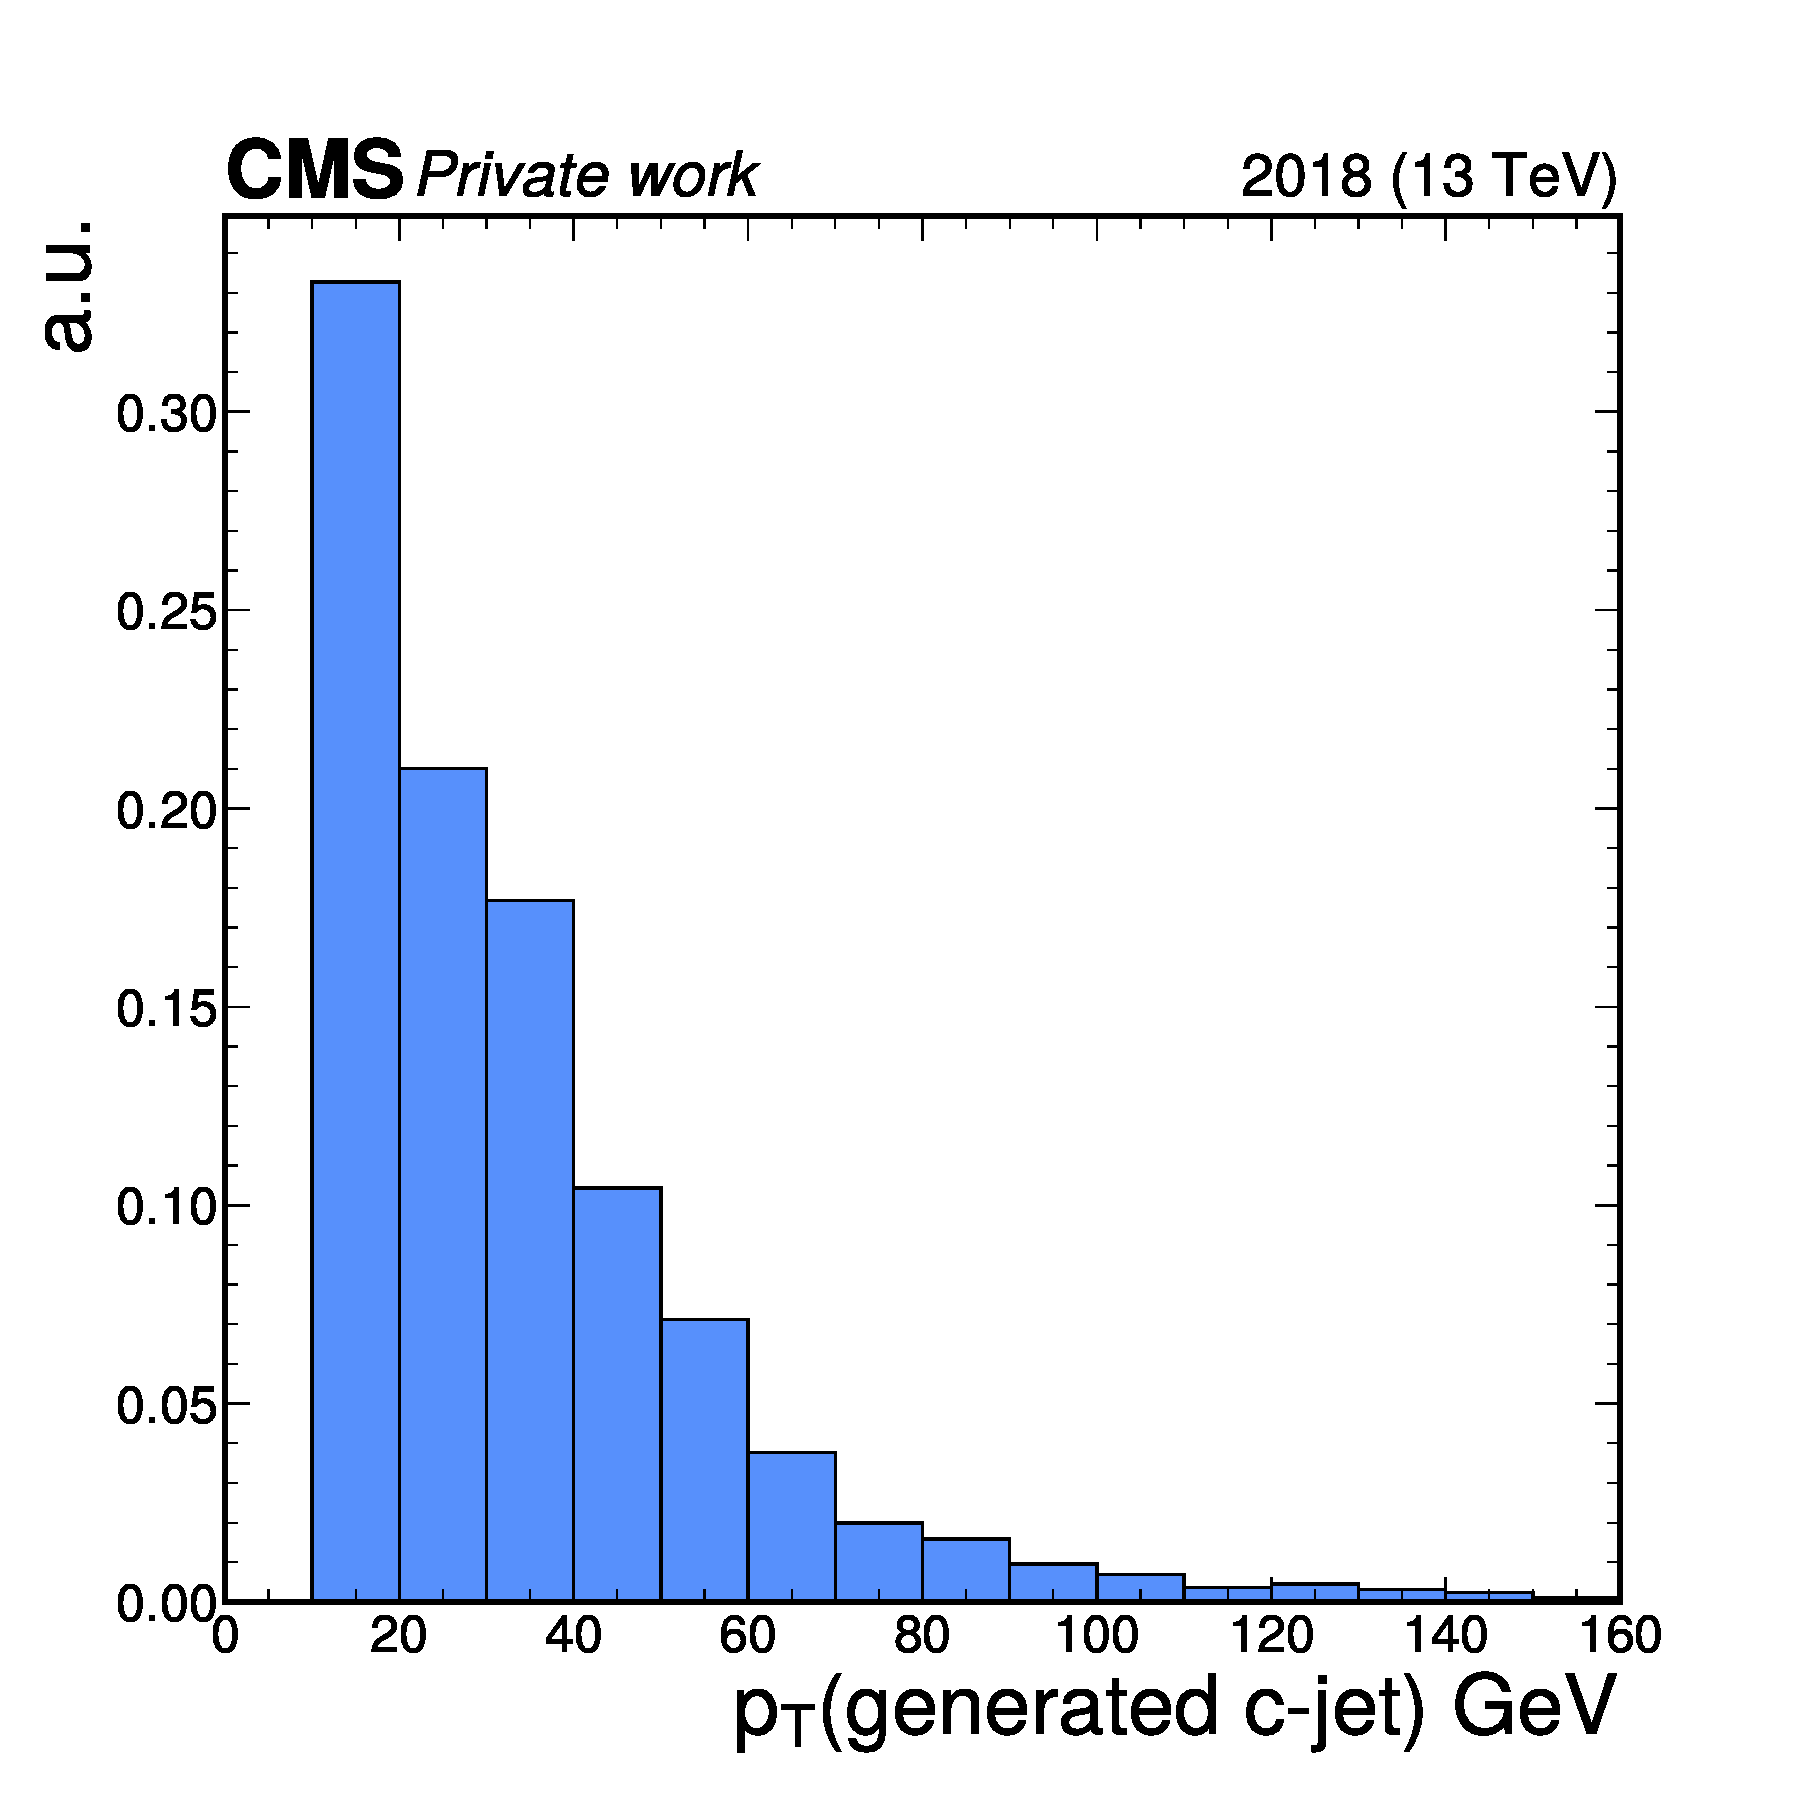
\includegraphics[width=0.5\textwidth]{figures/genPartonPt.pdf}
    \caption{The transverse momentum of the generator level, charm quark-initiated jet, which is generated in a \textsf{Madgraph5\_aMC$@$NLO} \cite{MadGraph} simulation of the cH process within the CMS detector. This typically takes on small values, as the observed spectrum falls steeply with increasing transverse momentum of the jet. Note that the cut-off that can be seen at 10 GeV is not a physics effect. Rather, the reason for this is that at very low transverse momenta, jets cannot be well-reconstructed experimentally and as such, a minimum transverse momentum requirement is applied during simulation.}
    \label{fig:JetPtcH}
\end{figure}

\subsection{The $\kappa$-framework}
\label{sec:kappaframework}
The $\kappa$-framework \cite{HiggsHandBook} is a commonly used framework to parametrise modifications to the couplings between the Higgs boson and other particles with respect to the expected SM values. It introduces the coupling modifier for the charm-Yukawa coupling as
\begin{align}
    \kappa_{c} = \frac{y_{c}}{y_{c}^{\mathrm{SM}}},
\end{align}
where $y_{c}$ is the measured Yukawa coupling and $y_{c}^{\mathrm{SM}}$ is the expected Yukawa coupling of the SM, calculated from the known charm quark mass. Accordingly, modifications to the Yukawa coupling of the charm quark are parametrised in this way as deviations from $\kappa_{\mathrm{c}} = 1$. However, $y_{\mathrm{c}}$ is not a quantity that can be measured directly. Instead, a signal strength measurement $\mu_{if}$ relative to the SM expectation, where $i$ represents the production process and $f$ represents the decay process, is made. As a result, a measurement of $\mu_{if}$ must be converted into an interpretation of $\kappa_{\mathrm{c}}$. This is a step that contains some finer subtleties. \\
\\
As described in \cite{PhysRevD.100.073013}, the rate of a Higgs production and decay process in relation to the expected SM signal (i.e. a signal strength) may be written as
\begin{align}
    \mu_{if} = \frac{\sigma_i \mathcal{B}_f}{(\sigma_i \mathcal{B}_f)^{\mathrm{SM}}}, \label{RateExpression}
\end{align}
\\
where $\sigma_i$ is the production cross section in a given channel $i$ and $\mathcal{B}_f$ is the decay branching ratio in a given channel $f$. This can alternatively be expressed as 
\begin{align}
    \sigma_i \mathcal{B}_f = \kappa_{r, i}^2 \sigma_i^{\mathrm{SM}} \frac{\kappa_f^2 \Gamma_f^{\mathrm{SM}}}{\Gamma_{\mathrm{H}}},
\end{align}
where modifications with respect to the SM expectation are introduced via the modifiers $\kappa_{r, i}$ and $\kappa_f$. The former modifies the SM production cross section $ \sigma_i^{\mathrm{SM}}$, while the latter modifies the partial SM decay width $\Gamma_f^{\mathrm{SF}}$ in the given decay mode. These decay widths can be understood as quantities that are inversely proportional to a particle's mean lifetime, which is dependent on the decay mode. As a result, they can be used to characterise the branching ratios with which a particle decays. The denominator $\Gamma_{\mathrm{H}}$, represents the total, summed decay width and can be written as
\begin{align}
    \Gamma_{\mathrm{H}} =& \Gamma_{\mathrm{H}}^{\mathrm{SM}}(\kappa_\mathrm{b}^2\mathcal{B}\mathrm{_{bb}^{SM}} + \kappa_\mathrm{W}^2\mathcal{B}\mathrm{_{WW}^{SM}} + \kappa_\mathrm{g}^2\mathcal{B}\mathrm{_{gg}^{SM}} + \kappa_\mathrm{\tau}^2\mathcal{B}\mathrm{_{\tau\tau}^{SM}} + \kappa_\mathrm{Z}^2\mathcal{B}\mathrm{_{ZZ}^{SM}} + \kappa_\mathrm{c}^2\mathcal{B}\mathrm{_{cc}^{SM}} \nonumber \\
    \quad& + \kappa_\mathrm{\gamma}^2\mathcal{B}\mathrm{_{\gamma\gamma}^{SM}}+ \kappa_\mathrm{Z\gamma}^2\mathcal{B}\mathrm{_{Z\gamma}^{SM}} + \kappa_\mathrm{s}^2\mathcal{B}\mathrm{_{ss}^{SM}} + \kappa_\mathrm{\mu}^2\mathcal{B}\mathrm{_{\mu\mu}^{SM}}) \label{TotalModifiedWidthSum} \\
    \vcentcolon=& \Gamma_{\mathrm{H}}^{\mathrm{SM}} \kappa_\mathrm{H}^2 \label{TotalModifiedWidth}
\end{align}
Here, $\Gamma_{\mathrm{H}}^{\mathrm{SM}}$ is the total decay width of the Higgs boson in the SM and the $\mathcal{B}_f^{\mathrm{SM}}$ are the branching ratios of the possible decay modes. Note that the coupling of the Higgs boson to a pair of gluons or photons, which are induced via a loop similar to that shown in \autoref{fig:cHFeynmanInsensitive}, are included as independent quantities. Again, each partial width contribution to the total width comes with a modifier $\kappa_i$. Substituting these expressions into \autoref{RateExpression}, the general rate modifier may be rewritten as
\begin{align}
    \mu_{if} = \frac{\kappa_{r,i}^2 \kappa_f^2}{\kappa_{\mathrm{H}}^2}. \label{RateExpressionSimplified}
\end{align}
\\
Now, assuming that only modifications to the charm-Yukawa coupling play a role in Higgs boson production, and no modifications are made to the decay mode (e.g. H $\rightarrow$ ZZ $\rightarrow$ 4$\mu$), \autoref{RateExpressionSimplified} becomes
\begin{align}
    \mu_{if} = \frac{\kappa_{\mathrm{c}}^2}{\kappa_{\mathrm{H}}^2} \label{RateExpressionForC}
\end{align}
for a signal strength measurement of the \cHZZ process component that is sensitive to \kappac. This component is henceforth denoted as \cHZZsen and is considered to be the process of interest. \\
\\
Using the flat direction approach discussed in \cite{PhysRevD.100.073013} and \cite{PhysRevD.103.095023}, a simplification of $\kappa_{\mathrm{H}}$ can be introduced. This approach is based on the finding that, when performing fits to existing Higgs boson production and decay rates, increases in the Yukawa couplings of light quarks (including the charm quark) can be compensated by increases in the couplings of the gauge bosons and heavy fermions. This is referred to as a ``flat direction" in the fit, for which observed Higgs boson production and decay rates can be modeled equally well for any value of $\kappa_{\mathrm{c}}$ by a respective scaling of all other processes. The individual modifiers in the sum of \autoref{TotalModifiedWidthSum}, with the exception of \kappac, as well as the modifiers in the nominator of \autoref{RateExpressionSimplified}, can thus be replaced with a single modifier $\kappa$. This allows \autoref{RateExpressionSimplified} to be expressed as
\begin{align}
    \mu_{if} = \frac{\kappa^4}{\kappa^2(1 - \mathcal{B}\mathrm{^{SM}_{cc}}) + \kappa_{\mathrm{c}}^2\mathcal{B}\mathrm{^{SM}_{cc}}},
\end{align}
for the described scaling of Higgs production and decay with $\kappa$. This expression, for some measured $\mu$, has a solution for $\kappa$ given by
\begin{align}
    \kappa^2 = \frac{(1 - \mathcal{B}\mathrm{^{SM}_{cc}})\mu}{2} + \frac{\sqrt{{(1 - \mathcal{B}\mathrm{^{SM}_{cc}})^2\mu^2} + 4\mu\mathcal{B}\mathrm{^{SM}_{cc}\kappa_{\mathrm{c}}^2}}}{2}. \label{GeneralKappa}
\end{align}
\\
Here, the expected SM decay width $\mathcal{B}\mathrm{^{SM}_{cc}} = 0.03$ can be substituted. Additionally, the fact that observed Higgs boson rates have been well measured to be close to their expected values (see e.g. \cite{HiggsRateMeasurementsCMS}) can be reflected by setting $\mu \approx 1$. As a result, only a dependence on $\kappa_{\mathrm{c}}$ remains in the expression. Thus, by replacing $\kappa_{\mathrm{H}}$ in \autoref{RateExpressionForC} with \autoref{GeneralKappa}, a final expression relating a measured signal strength of the \cHZZsen process to $\kappa_{\mathrm{c}}$ is obtained, given by

\begin{align}
    \mu_{\sigma_{\mathrm{cH}}\mathcal{B}\mathrm{(H\rightarrow ZZ)}_{\kappa_c}} = \frac{2\kappa_{\mathrm{c}}^2}{0.97 + \sqrt{(0.97)^2 + 4\cdot0.03\kappa_{\mathrm{c}}^2}}.
\end{align}
\\
Rearranging for $\kappa_{\mathrm{c}}$ gives
\\
\begin{align}
    \kappa_{\mathrm{c}} = \pm \sqrt{0.97\mu_{\sigma_{\mathrm{cH}}\mathcal{B}\mathrm{(H\rightarrow ZZ)}_{\kappa_c}} + 0.03\mu_{\sigma_{\mathrm{cH}}\mathcal{B}\mathrm{(H\rightarrow ZZ)}_{\kappa_c}}^2}.
\end{align}
\\
Effectively, this approach to interpreting $\kappa_{\mathrm{c}}$ from a signal strength measurement $\mu_{\sigma_{\mathrm{cH}}\mathcal{B}\mathrm{(H\rightarrow ZZ)}_{\kappa_c}}$ ensures compatibility with existing Higgs boson measurements. This is achieved by connecting the scaling behaviour of the \kappac-sensitive cH process with respect to \kappac \,, to the scaling of inclusive Higgs boson production rates and the total decay width of the Higgs boson. As a result, a slight modification of the quadratic relationship one might naively expect between \kappac\, and $\mu_{\sigma_{\mathrm{cH}}\mathcal{B}\mathrm{(H\rightarrow ZZ)}_{\kappa_c}}$ is obtained.

\section{The cH process in an EFT context}
\label{sec:cHEFT}
The cH process may also be interpreted in the context of Standard Model Effective Field Theory (SMEFT). In SMEFT, potential effects from physics processes not described by the SM (commonly referred to as beyond-the-SM or BSM physics) are parametrised in a mostly model-independent way. Specifically, the SMEFT framework can be used at colliders with a characteristic energy scale $E$ to describe the effects of processes with a characteristic energy scale above $E$. This concept is illustrated in \autoref{fig:EFT}. \\
\begin{figure}
    \centering
    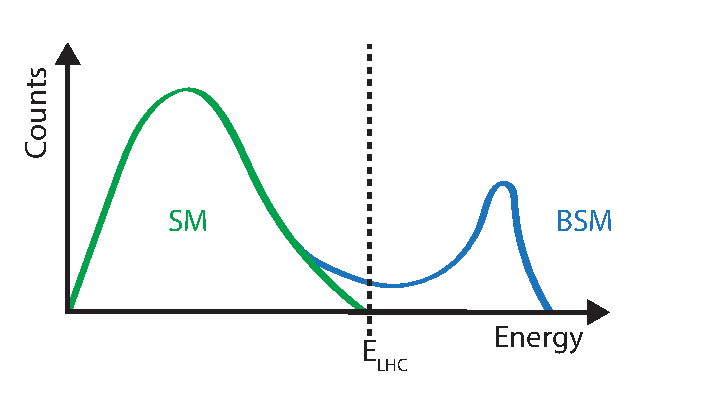
\includegraphics[width=0.8\textwidth]{figures/EFTDiagram.pdf}
    \caption{Illustration of how the presence of BSM physics, which is primarily visible beyond the reach of current collider energies (e.g. E$_{\mathrm{LHC}}$), can lead to subtle modifications of SM observables. These effects can be parametrised by SMEFT.}
    \label{fig:EFT}
\end{figure}
\\
Formally, SMEFT is a collection of all possible combinations of field interactions that obey the gauge invariance conditions of the SM. Generically, this can be expressed as an expansion in the energy scale of the new physics $\Lambda$ 
\\
\begin{align}
    \mathcal{L_{\mathrm{SMEFT}}} = \mathcal{L_{\mathrm{SM}}} + \sum_{d > 4} \sum_i \frac{C_i}{\Lambda^{d-4}} \hat{O}_i^d \label{EFTEquation}
\end{align}
\\
where $\mathcal{L_{\mathrm{SM}}}$ is the SM Lagrangian density, $O_i^d$ denotes a particular operator (i.e. a particular combination of fields) with a dimensionless coupling coefficient $C_i$ (typically referred to as Wilson coefficients) and $d$ denotes the dimension of the operator. The dimensionality is derived through a dimensional analysis of a Lagrangian and its fields, where energy dimensions of terms may be deduced from the requirement that the action
\\
\begin{align}
    \mathrm{S} = \int \mathcal{L} \, d^4x
\end{align}
\\
remains dimensionless. Accordingly, $\mathcal{L_{\mathrm{SM}}}$ is of energy dimension four. Since the SMEFT operators $O_i^d$ all have energy dimensions higher than four and $\Lambda$ comes with energy dimension one, the terms in the sum of \autoref{EFTEquation} are scaled with 1/$\Lambda^{d-4}$ to ensure the combination also has an energy dimension of four. \\
\\
Typically, operators in SMEFT are grouped by their energy dimension. In $d=5$, only one possible operator exists that violates lepton number \cite{Weinberg:1979sa} and is not relevant in this work. In $d=6$ however, a plethora of valid operators exist. These are commonly described in the Warsaw basis \cite{WarsawBasis}, which is representation of $d=5$ and $d=6$ operators. In this basis, a total of 59 independent operators are found. Since $d=7$ operators again violate lepton number and each additional dimension adds a suppressive factor of $\Lambda^{-1}$, a simplified SMEFT schema is commonly used in which only the contribution of $d=6$ operators is considered in the expansion. Thus, \autoref{EFTEquation} simplifies to 

\begin{align}
    \mathcal{L_{\mathrm{SMEFT}}} = \mathcal{L_{\mathrm{SM}}} + \sum_i \frac{C_i}{\Lambda^{2}} \hat{O}_i^{(6)} \label{EFTEQuationDim6}
\end{align}
\\
A good overview of SMEFT can be found in \cite{SMEFTOverview}.
\\
\subsection{The chromomagnetic dipole operator}
\label{sec:CMDOperator}

A particular operator relevant to this work is referred to as the chromomagnetic dipole (CMD) operator $\hat{O}_{qG}$, which introduces a four-particle interaction involving a Higgs boson, a gluon and a pair of quarks. For the charm quark, the CMD operator is written as 

\begin{align}
    \hat{O}_{cG} = (\overline{q}_{2, L} \sigma^{\mu\nu} T^ac)\tilde{\phi}G_{\mu\nu}^a. 
\end{align}
\\
Here, $\overline{q}_{2, L}$ is the second generation, left-handed quark doublet, $\sigma^{\mu\nu}$ = $i[\gamma_{\mu}, \gamma_{\nu}]/2$ with the Dirac matrices $\gamma_{\mu}$ , $T^a$ are the generators of the SU(3) symmetry group, c is the right-handed charm quark singlet, $\tilde{\phi}$ is the adjoint Higgs doublet and $G_{\mu\nu}^a$ is the field strength tensor of the strong interaction. This operator may be uniquely bounded with the cH process due its unique chiral structure, which mixes left and right-handed spinors. Such a structure is otherwise only found in the Yukawa and quark-Higgs boson interaction terms of the SM. \\
\\
To better understand this, it is worth considering other processes such as inclusive Higgs boson production, which have been successfully leveraged to set strong constraints on the top quark CMD operator $\hat{O}_{tG}$ \cite{CMSGlobalSMEFTFit}. Typically, the strategy that is used to probe even small Wilson coefficients, such as $C_{tG}$, is to exploit interference of the relevant (small) SMEFT contribution with a larger SM contribution. Though the pure SMEFT contribution itself may be small and experimentally negligible due to limited analysis sensitivity, the much larger contribution of the SM process it interferes with can result in a non-negligible interference effect with respect to the SM process. These interference effects occur when two processes are mediated in different ways, though they have the same initial and final states. However, the chiral structure of the CMD operator influences the effectiveness of this strategy. Since the $\hat{O}_{qG}$ operator effectively flips the chirality of the incoming and outgoing quarks, an additional \textit{chirality flip} must be inserted for the SMEFT contribution to produce interference with the SM process. This is visualised in \autoref{fig:CMDChirality}. Such a chirality flip is proportional to the mass $m_q$ of the respective quark. As a result, the interference contribution for a much lighter quark is significantly suppressed in comparison to the top quark, as also argued for the bottom quark in \cite{PhysRevD.93.053001}. Effectively, this means that the processes that prove effective in targeting $\hat{O}_{tG}$ due to the large mass of the top quark, are thus much less sensitive to $\hat{O}_{cG}$. However, since the cH process itself contains the chirality flipping quark-Higgs boson vertex, interference terms between the EFT and SM contributions do not suffer from the above described effect. Furthermore, due to the very low expected cross section of the cH process, the contributions originating purely from $\hat{O}_{cG}$ may be comparatively large with respect to the SM cH process, even at small values of $C_{cG}$. Accordingly, the cH process may be an excellent target to constrain $\hat{O}_{cG}$. 
\begin{figure}
    \centering
    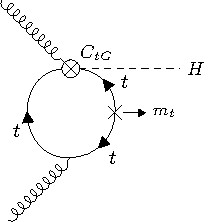
\includegraphics[width=0.3\textwidth]{figures/TopCMD.pdf}
    \caption{A modification of the gluon fusion process with a top quark loop by including the vertex introduced by the top quark CMD operator. Note that the arrows indicate chirality and not momentum flow. A chirality flip, denoted by the cross, proportional to the top quark mass $m_{t}$ is required for the inclusion of the top quark CMD vertex.}
    \label{fig:CMDChirality}
\end{figure}

\subsection{Validity of an EFT}
\label{sec:EFTValidty}
In addition to EFT terms needing to satisfy the gauge invariance conditions of the SM, two additional key validity conditions are typically required of an EFT. The first is related to the fact that in an EFT, the particle nature of e.g. new, heavy mediator particles is simplified into the introduction of a new effective vertex. For example, a 2$\rightarrow$2 particle resonant scattering via a new heavy mediator particle $\Omega$ associated with a newly introduced coupling constant $g_{*}$, is simplified via the introduction of a four-point interaction, as visualised in \autoref{fig:EFTMediatorToFourPoint}. This corresponds to a first-order approximation of the new particle's mediator as \\
\begin{align}
    \frac{g_{*}}{p^2 - m_{\Omega}} \quad \xrightarrow[m_{\Omega}^2 \gg p^2]{} \quad -\frac{g_{*}}{m_{\Omega}} \left( 1 + \frac{p^2}{m_{\Omega}^2} +  \frac{p^4}{m_{\Omega}^4} + ...  \right) \approx -\frac{g_{*}}{m_{\Omega}} 
\end{align}
\\
\begin{figure}
\begin{subfigure}{.4\textwidth}
    \centering
    \begin{tikzpicture}
    \begin{feynman}
        \vertex at (0, 1.5) (i1);
        \vertex at (0,-1.5) (i2);
        \vertex at (1.5, 0) (a);
        \vertex at (1, 0) (l1) {\(g_*\)};
        \vertex at (3, 0) (b);
         \vertex at (3.5, 0) (l2) {\(g_*\)};
        \vertex at (4.5, 1.5) (o1);
        \vertex at (4.5, -1.5) (o2);
        \vertex at (2.25,-0.3) () {\(\Omega\)};
        \diagram*{
            (i1) -- [fermion] (a),
            (i2) -- [fermion] (a),
            (a) -- [photon] (b),
            (b) -- [fermion] (o1),
            (b) -- [fermion] (o2);
        };
    \end{feynman}
    \end{tikzpicture}
\end{subfigure}%
\begin{subfigure}{.2\textwidth}
    \centering
    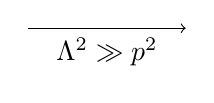
\begin{tikzpicture}
    \draw[->]        (1,-0.5)   -- (3,-0.5) node[midway,below] {\(\Lambda^2 \gg p^2\)};
    %\draw[>-Stealth] (0,0.3) -- (1,0.3);
    \end{tikzpicture}
\end{subfigure}
%\setcounter{subfigure}{3}%
\begin{subfigure}{.4\textwidth}
    \centering
    \begin{tikzpicture}
    \begin{feynman}
        \vertex[blob] (m) at (1.5, 0) {};
        \vertex at (0, 1.5) (i1);
        \vertex at (0,-1.5) (i2);
        \vertex at (1.5, 0) (a);
        \vertex at (2.3, 0) (l1) {\(\frac{g_*^2}{\Lambda^2}\)};
        \vertex at (3, 1.5) (o1);
        \vertex at (3, -1.5) (o2);
        \diagram*{
            (i1) -- [fermion] (m),
            (i2) -- [fermion] (m),
            (m) -- [fermion] (o1),
            (m) -- [fermion] (o2);
        };
    \end{feynman}
    \end{tikzpicture}
\end{subfigure}
\caption{Feynman diagrams depicting a resonant process in which the new mediator particle $\Omega$ is created (left) and the approximate description of this in an EFT, where the diagram is reduced to a four-point interaction.}
\label{fig:EFTMediatorToFourPoint}
\end{figure}%
For the EFT description of this simplification to be valid, the energy involved in processes containing the effective vertex introduced by the relevant operator must thus lie well below $m_{\Omega}$, which here represents the previously introduced new physics scale $\Lambda$. Practically, this can be achieved by placing an upper limit \mcut \, on the total energy that is considered in measurements of such processes. The requirement can be expressed as
\begin{align}
    M_{cut} < \Lambda . 
\end{align}
\\
A good estimator of \mcut \, is the invariant mass of the final state particles of a process. In case of the cH process, the invariant mass of the Higgs boson and jet system is a natural choice.\\
\\
The second condition that must be met is related to the perturbativity of the theory. Concretely, this means that higher dimensional operators should constitute increasingly smaller corrections, so that the sum of operator contributions converges. In the case of this work where only d=6 operators are considered, this means ensuring contributions from d=8 operators and higher are sufficiently small. While this cannot be determined with certainty without explicit knowledge of the underlying theory the EFT is estimating, a popular choice is to require that at most $g_{*} \sim 4\pi$ \cite{Elias_Mir__2013}. \\
\\
These two conditions may be combined into a single, simultaneous requirement. In \cite{Elias_Mir__2013}, an effective Lagrangian (ignoring relevant indices for simplicity) of the general form 
\begin{align}
\mathcal{L}_{\mathrm{eff}}=\frac{\Lambda^4}{g_*^2} \mathcal{L}\left(\frac{D_\mu}{\Lambda}, \frac{g_h \phi}{\Lambda}, \frac{g_{\psi_{L, R}} \psi_{L, R}}{\Lambda^{3 / 2}}, \frac{g F_{\mu \nu}}{\Lambda^2}\right)\,
\end{align}
\\
is obtained when a BSM coupling $g_{*}$ is introduced. This provides a prescription for the powers of the couplings and $\Lambda$ that are associated with the SM fields $\phi, \psi$ and $F_{\mu \nu}$, and the covariant derivate ${D_\mu}$. Here, $g$ represents the unaltered gauge field couplings of the SM, while $g_{\psi_{L, R}}$ and $g_h$ represent the coupling of SM fermion and the Higgs doublet to the BSM theory. In a single BSM coupling scenario, this simplifies to $g_{\psi_{L, R}} = g_h = g_*$. Applying this prescription to the CMD operator gives 

\begin{align}
    \hat{O}_{cG} \longrightarrow&
    \,\frac{\Lambda^4}{g^2_\star} \left[\left(\frac{g_\star \psi_{L,R}}{\Lambda^{3/2}}\right) \cdot \left(\frac{g_\star \psi_{L,R}}{\Lambda^{3/2}}\right) \cdot \left(\frac{g_\star \phi}{\Lambda}\right) \cdot \left(\frac{g_s G}{\Lambda^2}\right)\right] \\
    &= \frac{g_\star g_s}{\Lambda^2} \left( \psi_{L,R} \cdot \psi_{L,R}\cdot \phi \cdot G \right)\,. \label{CMDOperatorCoupling}
\end{align}
\\
Reading off from \autoref{CMDOperatorCoupling}, one can see that the coupling of the CMD operator is given by $g_\star g_s/\Lambda^2$. Comparing to \autoref{EFTEquation} thus reveals that the CMD Wilson coefficient is given by $C_{cG} = g_* g_s$. By requiring the first discussed validity condition, the relation 

\begin{align}
    \frac{C_{cG}}{\Lambda^2} < \frac{g_* g_s}{M_{cut}^2}
\end{align}
\\
is obtained. Since both $C_{cG}$ and $\Lambda$ are a priori unknown, we can redefine $\tilde{C}_{cG} = \frac{C_{cG}}{\Lambda^2}$. With this redefinition, and by setting $g_{*} \sim 4\pi$, the expression

\begin{align}
      \frac{\left| \tilde{C}_{cG} \right| M_{{cut}^2}}{4\pi g_s} < 1\,
\end{align}
\\
can be used to define a plane in $\tilde{C}_{cG}$ and \mcut \, that satisfies both of the previously discussed conditions. This plane is visualised in \autoref{fig:validityCMD}, showing regions in which the validity condition is (loosely) satisfied and in which it is not satisfied. Constraints placed on the CMD operator for a given \mcut\, value can be cross-checked against this to ensure the validity of the constraint. 

\begin{figure}
    \centering
    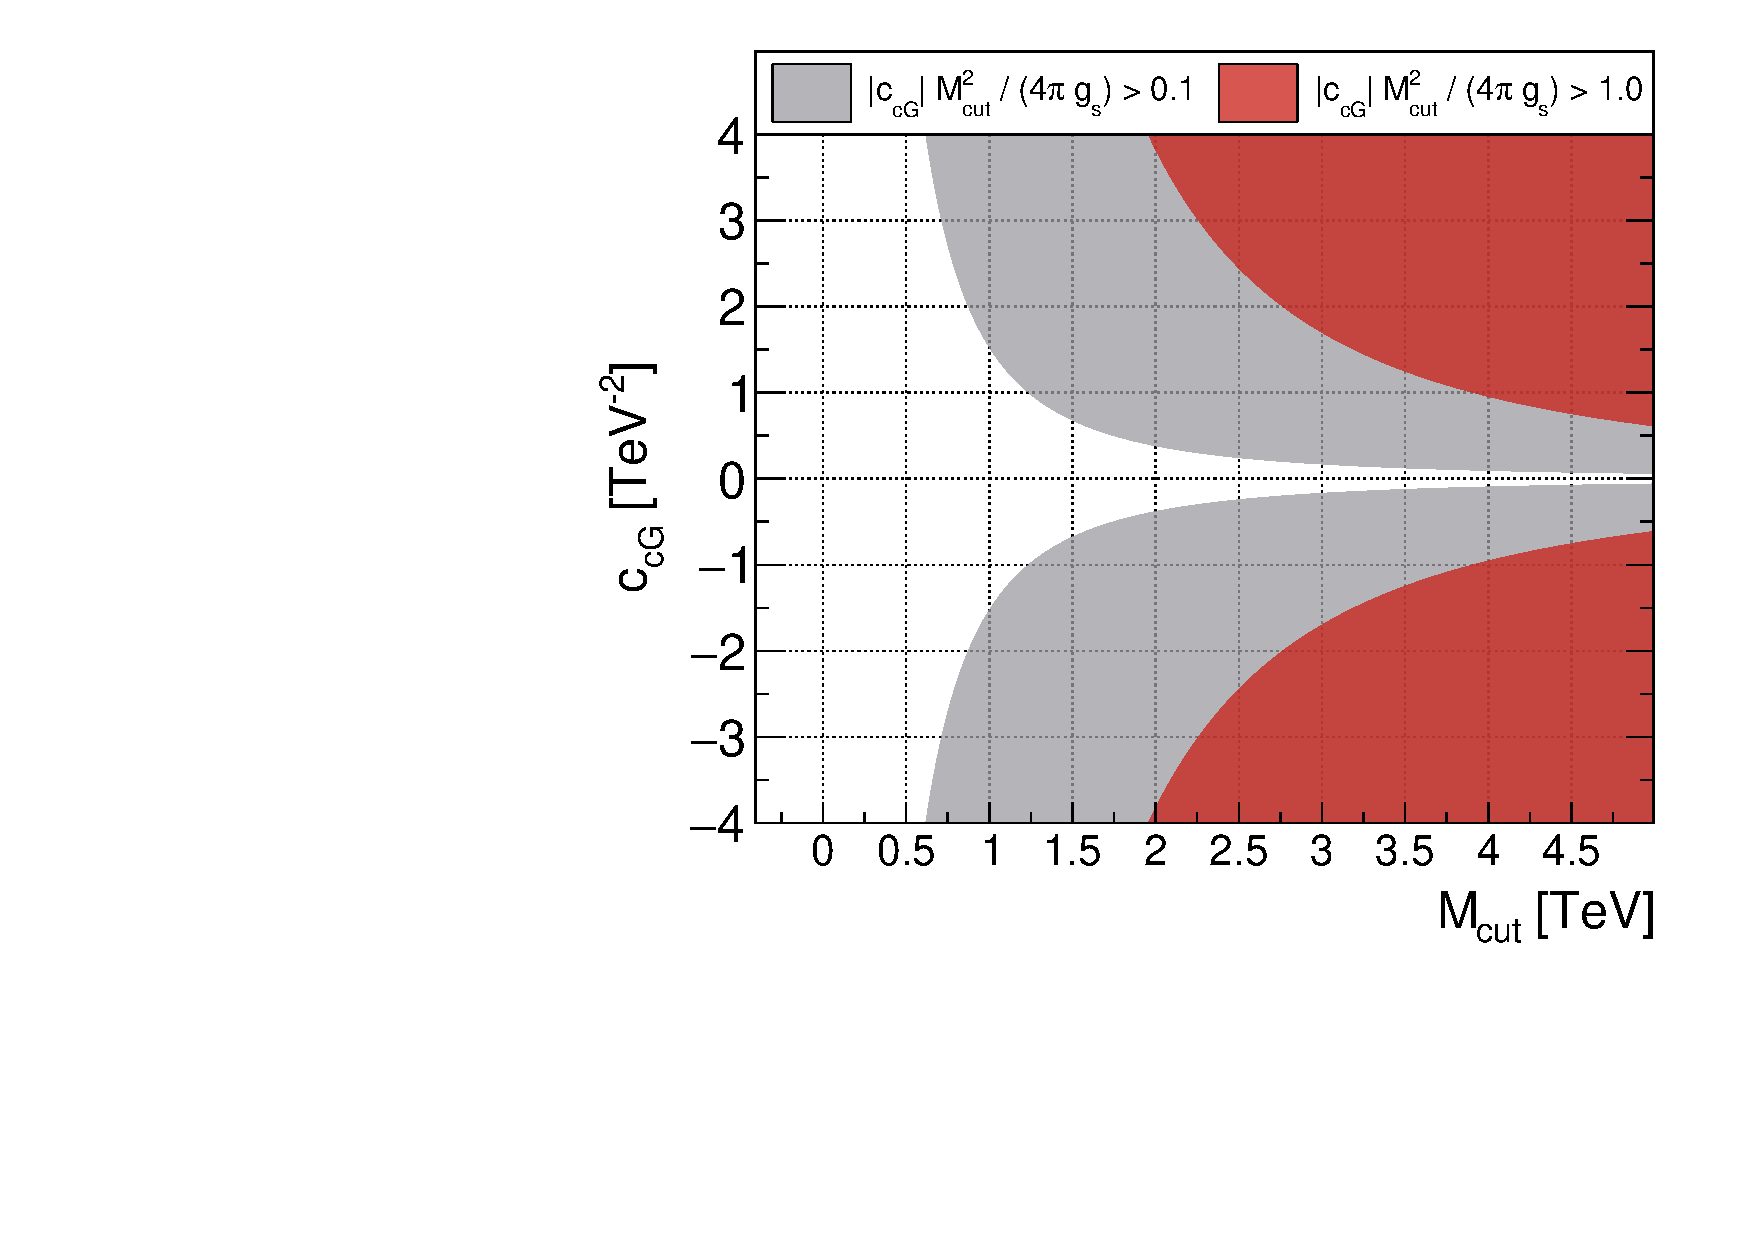
\includegraphics[width=0.6\textwidth]{figures/validityCMD.pdf}
    \caption{Diagram showing the plane spanned by $\tilde{C}_{cG}$ (here $\mathrm{c_{cG}}$) and \mcut \, for the CMD operator. The white region shows the region in which the perturbativity requirement is well satisfied. The grey region represents the transition from the white region to the red region, in which the perturbativity requirement is no longer valid. Figure taken from \cite{PhenoPaper} } 
    \label{fig:validityCMD}
\end{figure}

\section{State of the art on \kappac}
\label{SOAkappac}
Given the previously described status of the charm-Yukawa coupling in our current, experimental picture of the Higgs boson, analyses targeting the charm-Yukawa coupling are becoming of increased interest. This pertains particularly to the cH process, since it is considered a relatively novel process. In reflection of this, recent, first-time analyses of the cH($\gamma\gamma$) and cH(WW) channels using Run-2 data recorded by the CMS experiment have been published. The corresponding results of both analyses are interpreted in terms of the charm-Yukawa coupling modifier \kappac\, and upper limits on \kappac \, at 95\% CL are reported at $\mid$\kappac$\mid$ = \, 38.1 for cH($\gamma\gamma$) \cite{cmscHgammgamma} and $\mid$\kappac$\mid$ = \,211 for cH(WW) \cite{cmscHWW}, respectively. The ATLAS collaboration has similarly recently published an analysis of the cH($\gamma\gamma$) channel using Run-2 data \cite{cHATLAS}. However, only inclusive cH production is considered in this analysis. A measured inclusive cH cross section of 5.3 pb is reported and no direct interpretation with respect to \kappac\ is made. \\
\\
While the methods used to reconstruct Higgs boson decays in the cH($\gamma\gamma$), cH(WW) and also H(ZZ$\rightarrow4\ell$) channels are well established \cite{HWWPaper}\cite{HgammagammaPaper}\cite{HIG19-001}, procedures with which to identify the associated charm quark-initiated jet of the cH process may yet be optimised. In both the existing cH($\gamma\gamma$) and cH(WW) analyses, this task is accomplished by performing a comparatively simple selection of jet candidates based on fixed discriminator thresholds that are obtained from jet flavour-tagging algorithms (these are introduced in \autoref{sec:charmTagging}). Given that the identification of charm quark-initiated jets via such methods remains to be relatively inefficient, the development of alternative methods is of significant interest and are explored in this work. A potential ansatz to this is performing a kinematics-based jet association that is agnostic towards jet flavour. Such an algorithm is devised in this work and is detailed in \autoref{sec:JetCandidateSelection}. This, in turn, also enables the use of the full spectrum of the jet flavour-tagging discriminator of the selected jet in a final statistical evaluation, as is described in \autoref{sec:SMResult}. Such an alternative approach to identifying an associated charm-quark initiated jet could improve experimental sensitivity to the cH process. The reason for this is that the previous cH($\gamma\gamma$) and cH(WW) analysis efforts report large statistical uncertainties, as is expected when targeting processes with very low cross sections such as the cH process. As a result, approaches with a more inclusive jet selection method may improve analysis sensitivity, given that cH process contributions in which the associated charm quark-initiated jet cannot be well identified by jet-flavour identification methods are thus no longer discarded and may still contribute in a final statistical evaluation. \\
\\
Also of note are the significant theoretical uncertainties associated with the current modelling of the cH process, which affects all analyses of the cH process independently of the decay mode of the Higgs boson. This includes an uncertainty originating from the modelling of the charm quark mass when the charm-quark originates from the proton, as well as more generally the modelling of the emission of massive quarks alongside a Higgs boson. The former is captured via a so-called \textit{flavour scheme uncertainty}, as detailed in \autoref{sec:cHSimulation}, while the latter is described in \autoref{sec:IrreducibleBackgrounds}. These uncertainties are found to be leading systematic uncertainty sources in the cH($\gamma\gamma$) and cH(WW) channels, and thus are similarly expected to significantly impact an analysis of the cH(ZZ$\rightarrow4\mu$) channel. Improvements to these aspects of the process modelling thus remain to be of significant interest and potential approaches are discussed in \autoref{sec:SMAnalysisImprovements}. \\
\\
As previously suggested, it is also possible to constrain \kappac \, using more indirect methods. Significant deviations of the Yukawa couplings of the light flavour quarks (up, down, strange, charm) for example can lead to deviations of the inclusive Higgs production cross section. Accordingly, such potential deviations have previously been explored by the CMS collaboration in an analysis of inclusive Higgs boson production in the H(ZZ$\rightarrow4\ell$) channel \cite{gammaHProduction} and a constraint of \kappac$\,\in[-3.8, 3.2]$ is reported at a 95\% CL. However, it should be noted that the interpretation with respect to \kappac \, that is made in such a way requires somewhat stronger signal modelling assumptions, since Higgs production can be modified in a variety of ways, including the modification of the Yukawa couplings of all other quark flavours. In practice, this means the Yukawa couplings of all other quarks must be set explicitly by hand in a fit, or simultaneously be allowed to take on best-fit values. Additionally, the inclusive Higgs boson production mechanisms must be assumed to be otherwise SM-like. Other, similar analyses have also been proposed, such as in \cite{Bishara_2017}, where the differential transverse momentum of the Higgs boson in inclusive Higgs boson production is also found to be sensitive to \kappac \, at a level similar to the sensitivity obtained in \cite{gammaHProduction}. \\
\\
The most stringent, direct constraints to date on \kappac \,, however, currently originate from analyses that target H(\ccbar) decays. The best example of this is a recent combination of the VH(\ccbar) and t$\overline{\mathrm{t}}$H(\ccbar) channels by the CMS collaboration, for which an observed 95\% CL upper limit of $\mid$\kappac$\mid$\,=\,3.5 is reported \cite{cmscollaboration2025simultaneousprobecharmquark}. The ATLAS collaboration is likewise able to set a similar 95\% CL upper limit of $\mid$\kappac$\mid$ = 4.2, in an analysis of the VH(\ccbar) channel \cite{VHATLAS}. Additionally, the result of a first-time analysis of inclusive H(\ccbar) decays by the LHCb collaboration also looks promising \cite{LHCbCC}. In this analysis, an upper limit of $\mid$\kappac$\mid$ = 43 is derived, though using a much smaller dataset, indicating that such an approach could also yield significant sensitivity to \kappac. The comparatively strong constraints on \kappac\, that are derived in these analyses may originate from the fact that the final state particles, particularly the charm quark-initiated jets originating from H(\ccbar) decays are associated with significantly higher transverse momenta than, for example, the associated charm quark-initiated jet of the cH process. As such, the reconstruction of these processes is less prone to detector acceptance effects associated with jets at low transverse momentum, as is the case for cH analyses. Though analyses targeting H(\ccbar) decays must deal with significantly larger QCD backgrounds due to the presence of two charm quark-initiated jets in the signal signature, this trade-off may still be favourable due to the low signal yields associated with all charm-Yukawa sensitive processes. Furthermore, analyses of the VH(\ccbar), t$\overline{\mathrm{t}}$H(\ccbar) and inclusive H(\ccbar) processes are not constrained by the significant flavour scheme uncertainty that affects the cH process. \\
\\ 
Though the constraints derived in the aforementioned cH($\gamma\gamma$) and cH(WW) analyses are thus comparatively weak with respect to the channels involving direct H(\ccbar) decays, or even the discussed indirect measurement methods, further analysis of the cH process nonetheless provide important complementary results. Moreover, analyses of the cH process may still contribute significantly in a statistical combination, especially since there are still significant analysis improvements to explore. This is especially important given that even at the High-Luminosity LHC (HL-LHC), the projected sensitivity to the charm-Yukawa coupling in individual channels is only starting to approach one \cite{PhysRevD.111.053003}. Accordingly, the development and improvement of well-understood analysis methods, together with a combination of analysis channels, are key facets to exceeding the expectations set by such a projection. By performing a first-time analysis of the previously unexplored \cHZZ channel, as well as exploring novel analysis methods that may also be applicable in other analysis channels of the cH process, this work intends to contribute to making such a future measurement of the charm-Yukawa coupling possible. Furthermore, SMEFT interpretations of the cH process, which may be associated with modifications of \kappac, remain entirely unexplored in an experimental context. As such, this work also seeks to make a first-time foray into such scenarios.